\documentclass[UTF8]{ctexart}

%固定图片位置
\usepackage{float}

%插入超链接
\usepackage{url}

\usepackage{tikz,mathpazo}
\usetikzlibrary{shapes.geometric, arrows}
\usetikzlibrary{calc}

%\usepackage[affil-it]{authblk}

\usepackage{listings}
%插入代码的配置
\definecolor{CPPLight}  {HTML} {686868}
\definecolor{CPPSteel}  {HTML} {888888}
\definecolor{CPPDark}   {HTML} {262626}
\definecolor{CPPBlue}   {HTML} {4172A3}
\definecolor{CPPGreen}  {HTML} {487818}
\definecolor{CPPBrown}  {HTML} {A07040}
\definecolor{CPPRed}    {HTML} {AD4D3A}
\definecolor{CPPViolet} {HTML} {7040A0}
\definecolor{CPPGray}  {HTML} {B8B8B8}
\lstset{
	language=Matlab,                                     % 设置语言
    columns=fixed,    
    breaklines = true,   
    basicstyle=\small ,
    numbers=left,                                        % 在左侧显示行号
    %frame=none,                                          % 不显示背景边框
    backgroundcolor=\color[RGB]{245,245,244},            % 设定背景颜色
    keywordstyle=\color[RGB]{40,40,255}\bfseries,                 % 设定关键字颜色
    %commentstyle=\color{red!10!green!70}\textit,    % 设置代码注释的颜色
    numberstyle=\tiny\color{darkgray},           % 设定行号格式
    commentstyle=\it\color[RGB]{0,96,96},                % 设置代码注释的格式
    stringstyle=\rmfamily\slshape\color[RGB]{128,0,0},   % 设置字符串格式
    showstringspaces=false,                              % 不显示字符串中的空格                           
    %morekeywords={True,alignas,continute,friend,register,true,alignof,decltype,goto,
    %reinterpret_cast,try,asm,defult,if,return,typedef,auto,delete,inline,short,
    %typeid,bool,do,int,signed,typename,break,double,long,sizeof,union,case,
    %dynamic_cast,mutable,static,unsigned,catch,else,namespace,static_assert,using,
    %char,enum,new,static_cast,virtual,char16_t,char32_t,explict,noexcept,struct,
    %void,export,nullptr,switch,volatile,class,extern,operator,template,wchar_t,
    %const,false,private,this,while,constexpr,float,protected,thread_local,
    %const_cast,for,public,throw,std,rand},
    emph={access,and,break,class,continue,def,del,elif ,else,%
	except,exec,finally,for,from,global,if,import,in,i s,%
	lambda,not,or,pass,print,raise,return,try,while, imshow, subplot, figure,%
    log, fft2, fftshift, abs, size, rgb2gray, imread},
    emphstyle=\color{CPPViolet}\bfseries, 
    emph={[2]True, False, None, self},
	emphstyle=[2]\color{green},
	emph={[3]from, import, as},
	emphstyle=[3]\color{blue},
	upquote=true,
	morecomment=[s]{"""}{"""},
    morecomment=[s]{\%}{},
	%commentstyle=\color{orange}\slshape,
    commentstyle=\color{red!10!green!70}\textit,    % 设置代码注释的颜色
	emph={[4]1, 2, 3, 4, 5, 6, 7, 8, 9, 0},
	emphstyle=[4]\color{red},
	emph={[5]numpy, np, plt},
	emphstyle=[5]\color{red},
	literate=*{:}{{\textcolor{blue}:}}{1}%
	{=}{{\textcolor{blue}=}}{1}%
	{-}{{\textcolor{blue}-}}{1}%
	{+}{{\textcolor{blue}+}}{1}%
	{*}{{\textcolor{blue}*}}{1}%
	{!}{{\textcolor{blue}!}}{1}%
	{(}{{\textcolor{blue}(}}{1}%
	{)}{{\textcolor{blue})}}{1}%
	{[}{{\textcolor{blue}[}}{1}%
	{]}{{\textcolor{blue}]}}{1}%
	{<}{{\textcolor{blue}<}}{1}%
	{>}{{\textcolor{blue}>}}{1},%
    %{\%}{{\textcolor{green}\%}}{1},%
	framexleftmargin=0.1mm, framextopmargin=0.1mm, frame=shadowbox, rulesepcolor=\color{black},
}



\usepackage{geometry}
\geometry{left=2cm, right=2cm, top=1.2cm, bottom=1.2cm}

%得到引用的标题内容
\usepackage{nameref} 

%添加首行缩进,两个字符
\usepackage{indentfirst}
\setlength{\parindent}{2em}

%多行公式一个编号
\usepackage{amsmath}

%文献引用,标准类型为plain
%\usepackage[hyperref=true,backend=biber,sorting=none,backref=true]{biblatex}
%\addbibresource{ref.bib}
\bibliographystyle{plain}
\usepackage{cite}

\pagestyle{plain}

%跨页表格
\usepackage{multirow}
\usepackage{longtable,booktabs}
\usepackage{supertabular}
\usepackage{makecell}

%调整itemize等的间距
\usepackage{enumitem}


\usepackage{graphicx}
\usepackage{subfigure}

%超链接
\usepackage[linkcolor=yellow,citecolor=red,backref=page,hyperfootnotes=true]{hyperref}
\hypersetup{
bookmarks=true,
colorlinks=true,
linkcolor=black
}
\usepackage{tabularx} %This package must be placed after package {hyperref}, otherwise footnote marks are NOT treated as hyperlinks.


%引入了一些改进的数学环境,如align
\usepackage{amsmath}

\title{数字图像处理报告四:傅里叶变换简述}
\author{姓名:鲁国锐 \protect\newline
\and 学号:17020021031 \\
\and 专业:电子信息科学与技术}
\date{2020年3月31日}

\begin{document}
	\maketitle
	\renewcommand{\contentsname}{目录}
	\renewcommand{\listfigurename}{插图目录}
	\renewcommand{\listtablename}{表格目录}
	\renewcommand{\refname}{参考文献}
	\renewcommand{\abstractname}{摘要}
	\renewcommand{\indexname}{索引}
	\renewcommand{\tablename}{表}
	\renewcommand{\figurename}{图}
	
	
	
	\tableofcontents
	\newpage
	
	\hypersetup{
	bookmarks=true,
	colorlinks=true,
	linkcolor=red,
	urlcolor=blue
	}
	\section{题目描述}
	\indent 以下左图为原图,右图是经傅里叶变换之后的频谱图,请解释频谱图与原图之间的对应关系。

			
			\begin{figure}[H]
				\centering 
				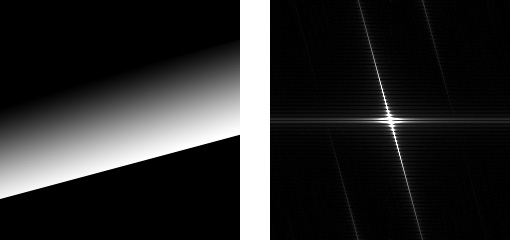
\includegraphics[scale=0.4]{org_img.png} 
				\caption{原图及其傅里叶变换} 
				\label{problem_img}
			\end{figure}
		


	
	\section{傅里叶变换}\label{Fourier_transform}
		\subsection{傅里叶变换历史}\label{傅里叶变换简述}
        \nocite{digit_image_Gonzalez}
        \nocite{signal_and_system}
        \nocite{discrete-time_signal_processing}
			\indent 傅里叶分析方法的建立有过一段漫长的历史,涉及到很多人的工作和许多不同物理现象的研究\cite{signal_and_system}。所谓的傅里叶分析中涉及的内容其实并非完全由傅里叶本人提出——欧拉在振动弦的研究中为其做出了许多奠基性的工作。在他之后又过了大半个世纪才由傅里叶提出“何周期信号信号都可以由正弦级数来表示”这一著名断言。在此之后,狄利赫里给出若干精确的条件,使得傅里叶级数得以严谨。由此我们也可以得到一个有趣的结论,傅里叶级数虽然以傅里叶的名字命名,但“傅里叶实际上并没有对傅里叶级数的数学理论做出什么贡献。然而,他确实洞察出这个级数表示法的潜在威力,并且在很大程度上正是由于他的工作和断言,才大大激励和推动了傅里叶级数问题的深入研究”\cite{signal_and_system}。
            
            \indent 前面所讲的研究都是关于数学物理学方面的,其研究对象主要集中在连续变量上,但另一个重要的数学分支——数值分析——的基础却是离散时间概念和方法\cite{signal_and_system}。对于离散序列的研究在$17$世纪的牛顿时代以及$18$、$19$世纪都有包括高斯在内的众多数学家为其做出贡献,可见对于离散信号的傅里叶分析有着一个完全不同的历史根基\cite{signal_and_system}。而$20$世纪$50$年代以来数字计算机的兴起,进一步激发了人们对于离散时间信号处理的兴趣。在此背景下,离散傅里叶变换($DFT$)作为一种有效的工具,其重要性愈加突出。但它所带来的高昂计算成本($O(N^2)$)却一直阻挡着$DFT$走向应用。
            
            \indent 这样的情况一直持续到$1965$年。在这一年,由$John\ Wilder\ Tukey$和$IBM$公司的$James\ Cooley$提出了“快速傅里叶变换($FFT$)”算法\cite{cooley1965algorithm},将时间复杂度降至$O(NlogN)$,使得以前出现的很多曾认为是不切实际的信号处理算法开始显露出具体实现的可能\cite{discrete-time_signal_processing}。因此,很多人把“数字信号处理”这门学科的创立时间定在了$1965$年。
%			\begin{enumerate}[leftmargin=50pt]
%				\item 光线透过镜头投射到感光元件表层;
%				\item 光线被感光元件表层上滤镜分解成不同色光;
%				\item 色光被各滤镜相对应的感光单元感知,并产生不同强度的模拟电流信号,再由感光元件的电路将这些信号收集起来;
%				\item 模拟信号通过模数转换器成为数字信号,再由$DSP$对这些信号进行处理,还原成为数字影像;
%				\item 数字影像被传输到存储卡上保存起来。
%			\end{enumerate}

		\subsection{傅里叶变换物理意义}
			\indent 直观来说,傅里叶变换其实是把一个信号投影到代表不同频率的正交基上($e^{j\omega}$,在时域中的基是$\delta(t)$);也可以理解成是从不同的角度来看待一个信号(如图\ref{time_vs_freq}所示)。
			
			\begin{figure}[htbp]
				\centering 
     			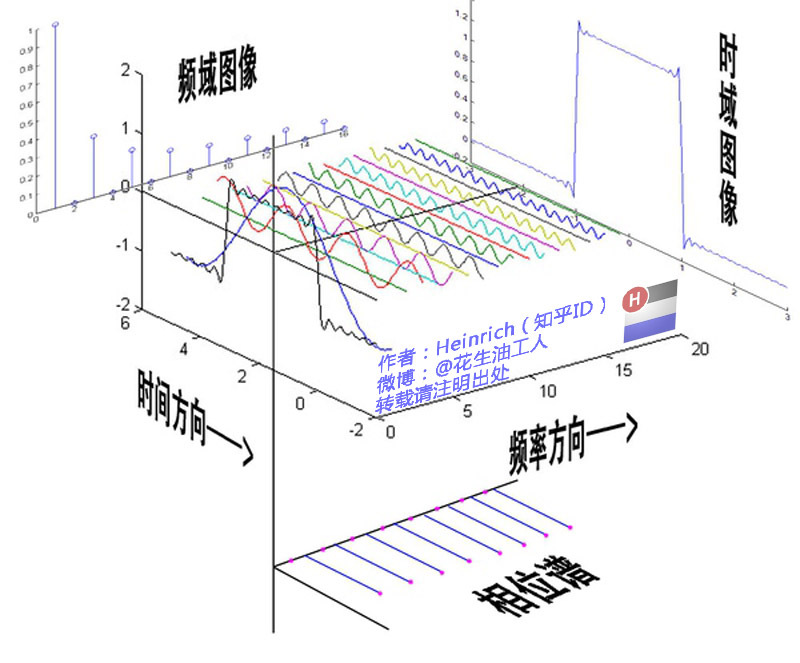
\includegraphics[scale=0.5]{time_vs_freq.jpg} 
				\caption{时域频域示意图} 
				\label{time_vs_freq}
			\end{figure}
            
            
            \indent 类比至二维情况下,我们仍然可以将一个二维信号(比如说图像)分解成不同频率的波。只不过现在分解得到的是平面波,相对于一维情况下又多了一个参量:方向(如图\ref{plane_wave}所示)。为了形象地表示幅度、方向等参量,我们引入二维情况下的频谱图。
            
            \begin{figure}[htbp]
            	\centering 
                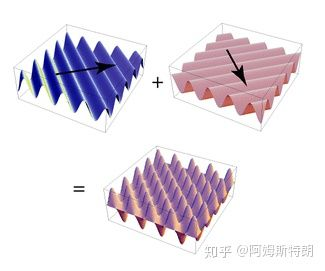
\includegraphics[scale=0.7]{plane_wave.jpg} 
            	\caption{平面波合成示意图} 
            	\label{plane_wave}
            \end{figure}
            
			 \indent 经过变换后的频谱图,中心处代表直流分量,靠近中心的位置代表低频分量,远离中心的则代表高频分量。每一个分量在频谱图上由一对关于原点对称的点表示,或者也可以说成是一对向量。这些向量的模(即到中心点的距离)代表了频率的高低,而相对于中心点的方向,则代表了波的方向,也就是图像变化的方向。而之所以是一对向量,是因为傅里叶变换后得到的是复数$e^{j2\pi(ut+vz)}$的系数,根据欧拉公式知道,一对共轭的$e^{jw}$才能合成一个正弦或余弦波,即正负频率分量叠加才得到一个正弦或余弦分量。而这个事实反映在频谱图上,就成了一对关于中心点对称的向量。


%			\indent 采取\ref{数字相机成像原理}节的方式,我们也可以把线性扫描相机的原理概括为以下$3$个步骤:
%			\begin{enumerate}[leftmargin=50pt]
%				\item 由条带传感器成像,给出一幅图像一行(或一列)的像素值;
%				\item 沿垂直于传感器带的方向移动一小段距离;
%				\item 重复步骤$1$和步骤$2$,直至整幅图像全部成像完毕。
%			\end{enumerate}

		
	\section{题目解释}\label{explanation}
		\indent 有了第\ref{Fourier_transform}节的铺垫,对题目所给图像的解释就有清楚许多。由图\ref{problem_img}中的左图可以看出,从左上到右下这个方向上像素值的跳变是最为激烈的,且在这个变化过程中有渐变,也有跳变,可以想见其频率成分应该会比较丰富。相应的,在频谱中可以看出,在该方向上有一条斜线,这代表在该方向上有许多不同频率的分量,与之前由空间域图像得到的猜想吻合。
        
        \indent 除了上述变化最剧烈的方向之外,沿其它方向的路径走,也会遇见像素值的变化,只是其变化的剧烈程度会小一些。再观察它对应的频谱图,能看到一条沿水平方向、比较亮的线,\textbf{但若放大仔细观察的话,还能发现有其它较暗的斜线},这些线相对于原点覆盖了很多其它方向;同时它们很暗这一事实,也与之前得出的在这些方向上变化程度较小这一结论想吻合。
%		\begin{enumerate}[leftmargin=50pt]
%			\item 所成图像在垂直方向上的大小不受限制;
%			\item 能够通过提高扫描频率达到非常高的分辨率;
%			\item 使用起来灵活方便等
%		\end{enumerate}
		
	\section{实验验证}
        \subsection{实验思想}
            \indent 从前面的分析可以看出,频谱图上的谱线与空间域中像素变化的方向及剧烈程度有关。从这个角度出发,如果把空间域图像转一个角度,频谱图中的谱线相应地也应该旋转相同的角度。我们将在之后的两个小节中对这个猜想进行验证。
        \subsection{实验代码}
            	\begin{lstlisting}[language=Matlab,caption={实验代码},label={broadcast.cpp}]
% reference: https://blog.csdn.net/jiugedexiaodi/article/details/79705308



img = imread('C:\Users\Asus-\Desktop\数字图像\report\04\rotate45.png');
img = rgb2gray(img);

% 将图像的数据格式转换为double型的,此时图像的数值范围由原来的[0,255],
% 变成了[0,1],其实不进行转换的话,也可以进行傅里叶变换,
% 只是傅里叶变换后的图像会有所不同
img=im2double(img);

% size(img)

F = fft2(img);
F = fftshift(F);
F = abs(F);

% 傅里叶变换后模值差异非常大,低频直流远远大于高频
% 不加这一句变换后的结果只能看到中间有一个亮点
T = log(1+F);
figure(1)
subplot(1, 2, 1)
imshow(img)
subplot(1, 2, 2)
% 后面的[],表示对图像做了一个类似于归一化的操作,
% 防止傅里叶变换后模值差异太大
imshow(T, [])
            	\end{lstlisting}
                
                
        \subsection{实验结果}
        
            \begin{figure}[htbp]
            	\centering 
                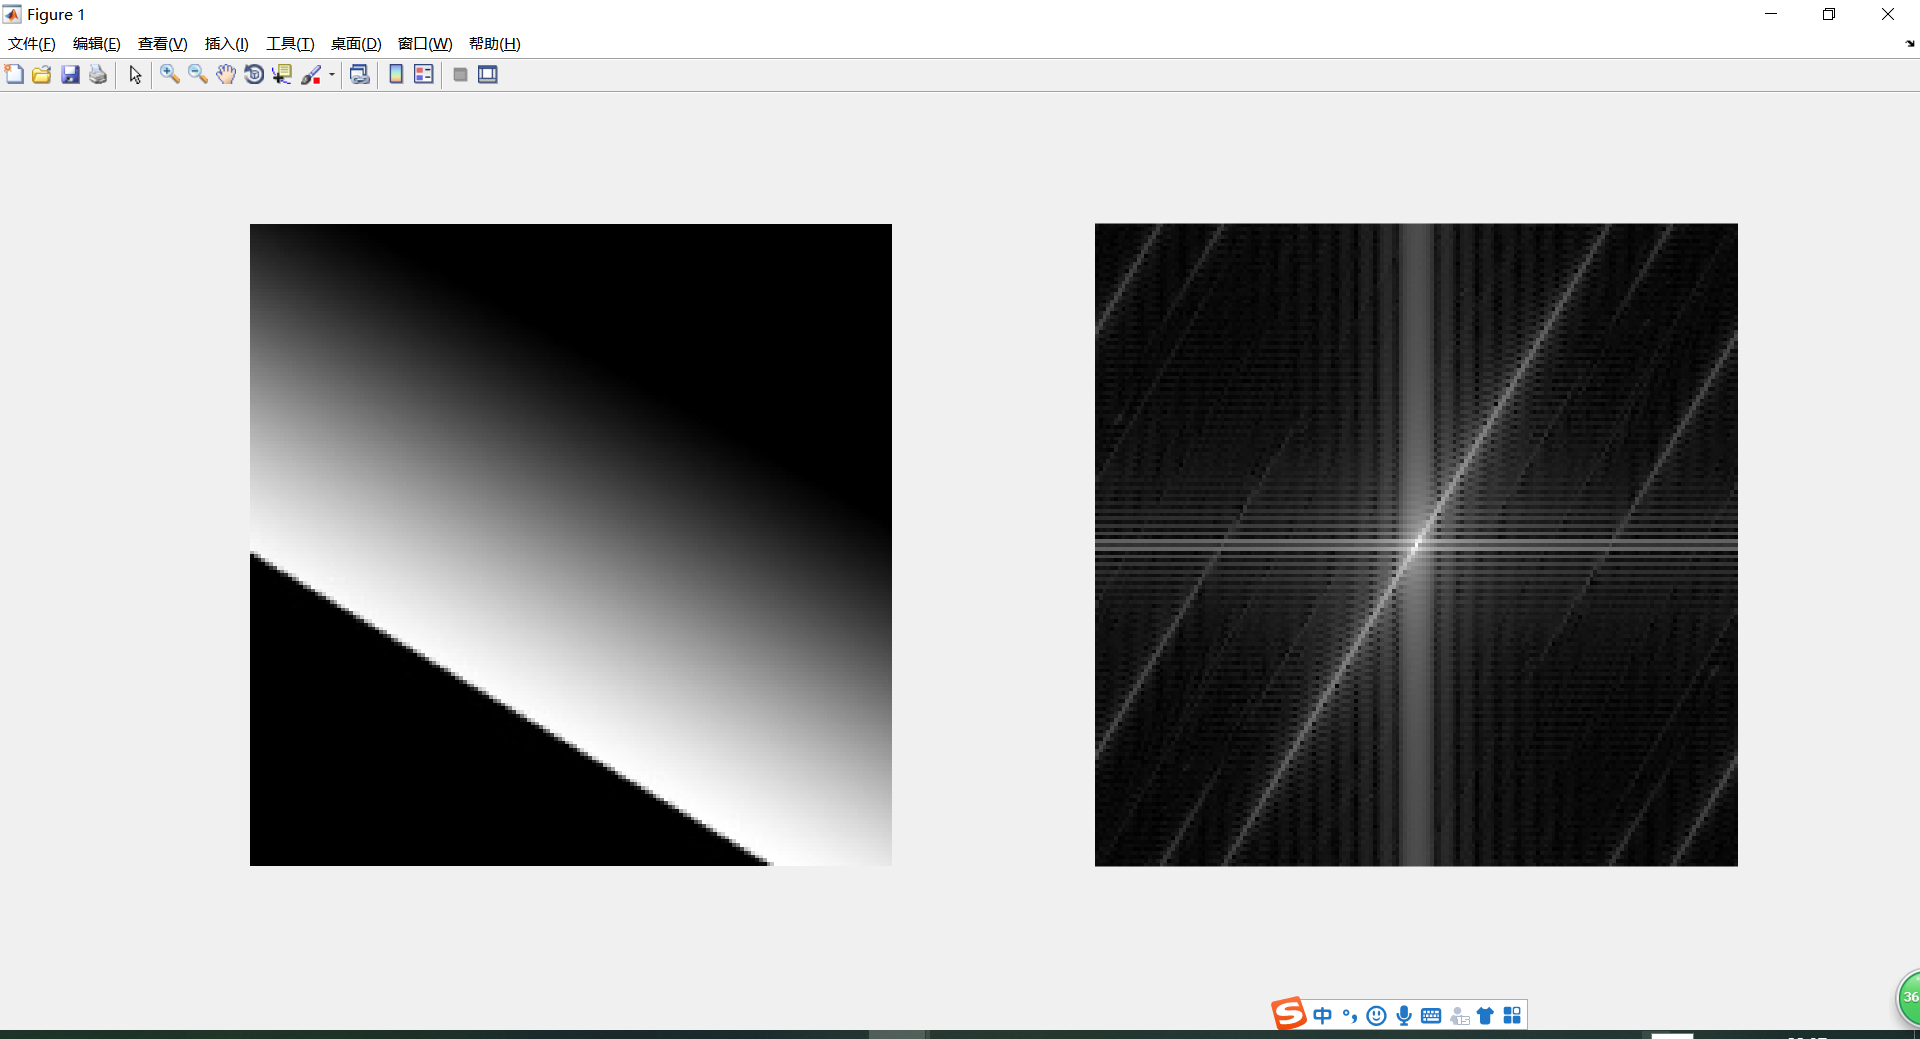
\includegraphics[scale=0.4]{result.png} 
            	\caption{实验结果} 
            	\label{result}
            \end{figure}
            \indent 从图中可以看出,基本符合预期。
            
            


	\section{总结}
		\indent 从结果可以看出,方向大体上符合预期,但也能看出相比题目给出的频谱,我们实验结果中又多了很多其它的分量。出现这些现象的原因可能是:空间域图像是由原图旋转再裁剪得到的,可能在裁剪图像的过程中导致图像某些部分有了变化,相当于引入了一些噪声,反映在频谱图中就是我们看到的这个效果了。
		
%			\begin{figure}[H]
%				\centering 
%				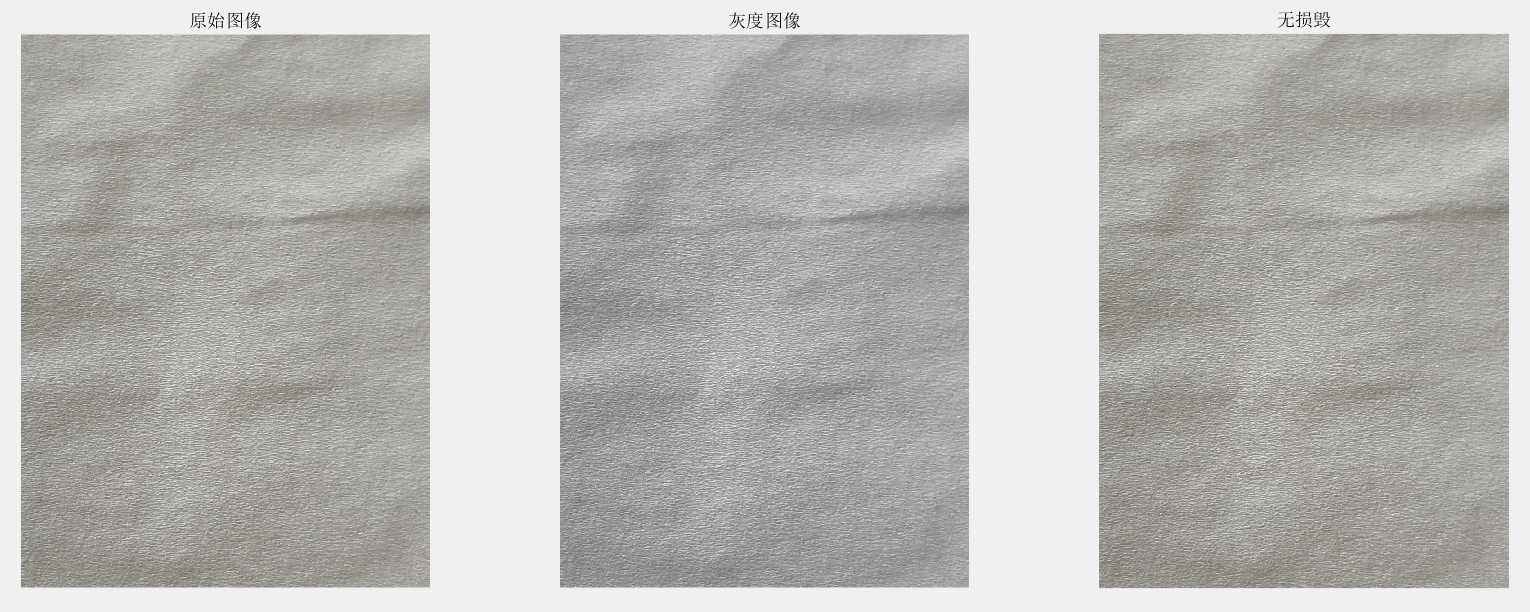
\includegraphics[scale=0.4]{res4.png} 
%				\caption{结果4} 
%				\label{res4}
%			\end{figure}
		

		
%			\begin{figure}[H]
%				\centering 
%				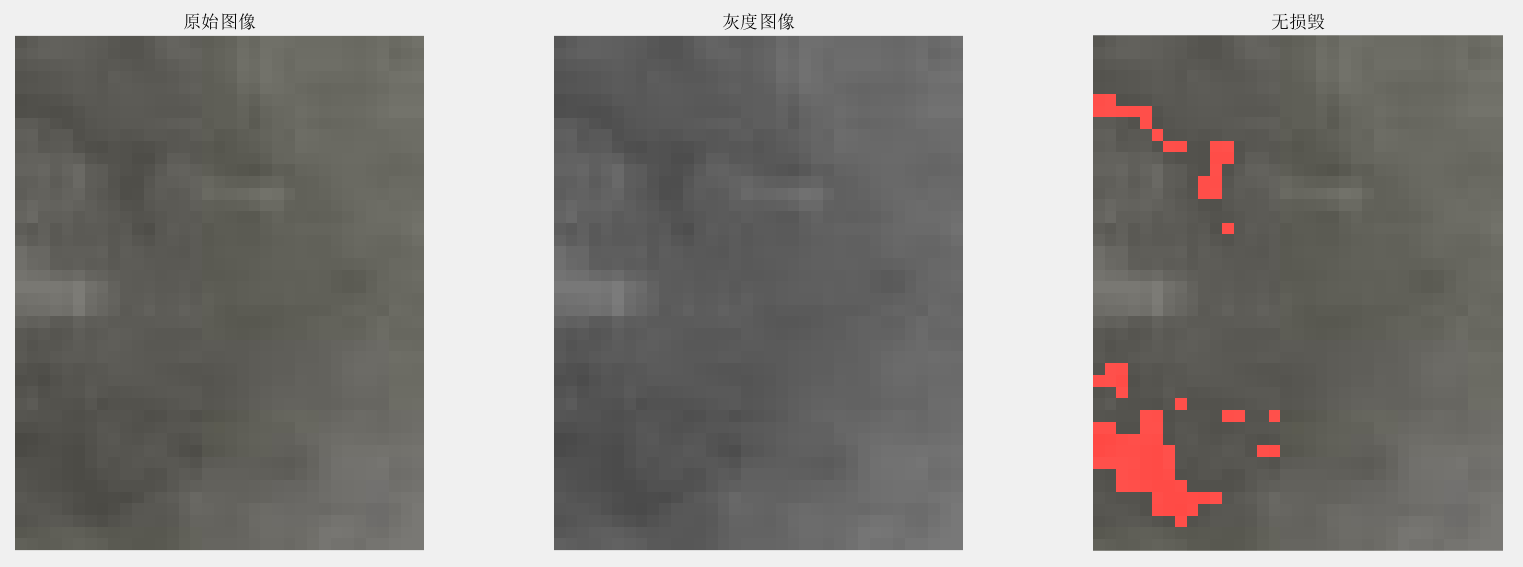
\includegraphics[scale=0.4]{res6.png} 
%				\caption{结果6(截取自结果5的阴影部分)} 
%				\label{res6}
%			\end{figure}
	
	
% 中文文献多个作者用中文逗号“,”连接
%\bibliography{ref.bib}
%\bibliographystyle{abbrv}
\bibliography{ref.bib}


\end{document}